%%%%%%%%%%%%%%%%%%%%%%%%%%%%%%%%%%%%%%%%%
%
% CMPT 435
% Spring 2019
% Lab One
%
%%%%%%%%%%%%%%%%%%%%%%%%%%%%%%%%%%%%%%%%%

%%%%%%%%%%%%%%%%%%%%%%%%%%%%%%%%%%%%%%%%%
% Short Sectioned Assignment
% LaTeX Template
% Version 1.0 (5/5/12)
%
% This template has been downloaded from: http://www.LaTeXTemplates.com
% Original author: % Frits Wenneker (http://www.howtotex.com)
% License: CC BY-NC-SA 3.0 (http://creativecommons.org/licenses/by-nc-sa/3.0/)
% Modified by Alan G. Labouseur  - alan@labouseur.com
%
%%%%%%%%%%%%%%%%%%%%%%%%%%%%%%%%%%%%%%%%%

%----------------------------------------------------------------------------------------
%	PACKAGES AND OTHER DOCUMENT CONFIGURATIONS
%----------------------------------------------------------------------------------------

\documentclass[letterpaper, 10pt]{article} 


\usepackage[english]{babel} % English language/hyphenation
\usepackage[utf8]{inputenc}
\usepackage{graphicx}
\usepackage[lined,linesnumbered,commentsnumbered]{algorithm2e}
\usepackage{listings}
\usepackage{minted}
\usepackage{fancyhdr} % Custom headers and footers
\pagestyle{fancyplain} % Makes all pages in the document conform to the custom headers and footers
\usepackage[table]{xcolor}
\usepackage{csquotes}
\usepackage{natbib}
\usepackage[nottoc]{tocbibind}
\usepackage{lastpage}
\usepackage{url}
\usepackage{float}
\usepackage{scrextend}
\usepackage{epigraph}
\fancyhead{} % No page header - if you want one, create it in the same way as the footers below
\fancyfoot[L]{} % Empty left footer
\fancyfoot[C]{page \thepage\ of \pageref{LastPage}} % Page numbering for center footer
\fancyfoot[R]{}
\usepackage{listings}% http://ctan.org/pkg/listings
\usepackage{hyperref}
\renewcommand{\headrulewidth}{0pt} % Remove header underlines
\renewcommand{\footrulewidth}{0pt} % Remove footer underlines
\setlength{\headheight}{13.6pt} % Customize the height of the header
\usepackage{pgfplots}

\pgfplotsset{width=7cm,compat=1.8}

%----------------------------------------------------------------------------------------
%	TITLE SECTION
%----------------------------------------------------------------------------------------

\newcommand{\horrule}[1]{\rule{\linewidth}{#1}} % Create horizontal rule command with 1 argument of height

\title{	
   \normalfont \normalsize 
   \textsc{CMPT 435 - Fall 2020 - Dr. Labouseur} \\[10pt] % Header stuff.
   \horrule{0.5pt} \\[0.25cm] 	% Top horizontal rule
   \large{Assignment Three -- Searching and Hashing} \\
   \textsc{Linear And Binary Search and an implementation of a Hash Table}\\[20pt]% Assignment title
 \author{Sam Alcosser \\ \normalsize Samuel.Alcosser1@Marist.edu}
   \horrule{0.5pt} \\ 	% Bottom horizontal rule
   


	% Today's date.
  
\date{\normalsize\today} 
}
\begin{document}




\fontfamily{bch}\selectfont
\maketitle
\tableofcontents
\newpage

\section{Introduction}

This document explains the implementations of linear search, binary search, and hash tables using C++. The organization of each section will generally follow the format of a brief explanation of the function, the code itself, and an explanation of the code with references to line numbers.


\section{the \texttt{randPick()} Function}

Most of the algorithms used in this program are reliant on the \texttt{randPick()} function, the routine used to generate the list of random elements.

\begin{center}
\textbf{Code Analysis}
\end{center}
\begin{addmargin}[-5em]{1em}
\begin{small}
\begin{minted}[linenos=true]{cpp}
oid Search::randPick(std::string mainArr[], std::string chosen[], int len, int lenOfChosen)
{

	int countTries = 0;

	for (int i = 0; i < lenOfChosen; i++)
	{

		bool same = true;
		while (same)
		{
			std::random_device dev; 
			std::mt19937 rng(dev());
			std::uniform_int_distribution<std::mt19937::result_type> dist6(0, len);

			std::string attempt = mainArr[dist6(rng)];
		
			bool foundSame = false;
			for (int j = 0; j < lenOfChosen; j++)	
			{

				if (chosen[j] == attempt)	

				{

					countTries++;
					foundSame = true;
					break;
				}
			}

			if (foundSame)
			{

				countTries++;	
				continue;
			}

			else
			{

				countTries++;
				chosen[i] = attempt;		
				same = false;
			}
		}
	}

	return;
}

\end{minted}
\end{small}
\end{addmargin}

\begin{enumerate}
    \item Begin a loop that will run an amount of times defined by the \texttt{lenOfChosen} variable, as was passed to the function.(line 6)
    \item After initializing a boolean variable called \texttt{same} to true, start a while loop that will complete once the variable is set to false. This will allow us to continue trying to generate random elements until an original element is found.(lines 9,10)
    \item Generate a random number between 0 and the length of the main array as defined by the \texttt{len} variable that was passed into the function. Retrieve the element at that index from array \texttt{mainArr[]}(lines 12-14).
    \item Set  a flag variable called \texttt{foundSame} to false.( line 18)
    \item Check if the element selected exists in the list of already chosen elements by looping through and checking each element with a loop.(lines 19-22)
    \item If the current element matches a previous one, set the \texttt{foundSame} flag, and break out of the for loop. With this the algorithm will stop the search.(lines 26-28)
    \item If the \texttt{foundSame} flag was set, reset the while loop and try generating a new number all over again.(lines 32-37)
    \item If there was not a same element, add that new item to the list of items and set the \texttt{same} flag to false. Now, the function will break out of the outer while loop.(lines 39-45)
\end{enumerate}


\section{Searching}

\subsection{Linear Search}

The linear search algorithm is a brute force algorithm used to retrieve data from a set of data. The algorithm simply starts at the beginning of the set, and tries each item until it finds what it is looking for.
\vspace{1em}
\begin{center}
    \textbf{Code Analysis}
\end{center}
\begin{addmargin}[-5em]{1em}
\begin{small}
\begin{minted}[linenos=true]{cpp}
int Search::linSearch(std::string mainArr[], int len, std::string chosen[], int lenOfChosen)
{
	std::cout << "---Linear Search---" << std::endl;
	int tCount = 0;

	for (int i = 0; i < lenOfChosen; i++)
	{
		int count = 0;
		for (int j = 0; j < len; j++)
		{
			if (mainArr[j] != chosen[i])
			{
				count++;
			}
			else
			{
				tCount += ++count;
				std::cout << "Found it at index " << j << " after " << count << " checks." << std::endl;

				break;
			}
		}
	}

	int avg = (int)(tCount / lenOfChosen);
	return avg;
}

\end{minted}
\end{small}
\end{addmargin}

As seen above, this algorithm really is quite simple.
\vspace{1em}


\begin{enumerate}
    \item Begin a loop from zero to the length, \texttt{lenOfChosen}, of the list of items \texttt{chosen[]},we would like to retrieve. (line 6)
    \item After initializing our temporary counter variable \texttt{count}, begin another loop from zero to the length, \texttt{len}, of the array \texttt{mainArr[]} which we are searching in. (line 9)
    \item If the item at the index defined by the inner loop does not match the item at the index defined by the outer loop (if the current item in the main array does not match the item we are searching for) increment our temporary count variable by one. (lines 11-14).
    \item Otherwise, meaning the items do match, increment the counter once more. Even though the item was found, this still counts as a comparison. Also, add the temporary counter \texttt{count} to the sum of \texttt{tCount}, which holds the total count of comparisons.(line 17)
    \item Since the item was found, end the inner for loop, and move onto the next item. (line 20)
    \item Once all items have been found, compute the average by dividing \texttt{tCount}, the total comparisons by \texttt{lenOfChosen}, the number of items searched for and return it from the function. (lines 25,26)
\end{enumerate}
\subsection{Binary Search}

Binary search is more complicated than linear search, but it is also much more efficient. To begin, binary search needs a sorted array. Without the array being sorted, the algorithm cannot function correctly. It is not shown within this document in full, as the purpose of this document is to explain searching and hashing, but the Merge Sort algorithm is used to sort the items prior to searching. 

\begin{center}
\includegraphics[width=\textwidth]{binSearch.png}
\end{center}
\textbf{Figure 1}

Once the array is sorted, binary search starts from the midpoint of the array, and depending on whether or not that midpoint value is greater than or less than the item being searched for, it will then switch to checking the lower half of the array or the higher half of the array. Once again, the same process will happen at that half of the array, and will continue to split the array and search until the item is found.
\newpage
\begin{center}
  \textbf{Code Analysis}  
\end{center}

\begin{addmargin}[-5em]{1em}
\begin{small}
\begin{minted}[linenos=true]{cpp}
int Search::binSearch(std::string mainArr[], int len, std::string chosen[], int lenOfChosen)
{
	std::cout << "---Binary Search---" << std::endl;
	int tCount = 0;

	for (int x = 0; x < lenOfChosen; x++)
	{

		int count = 0;
		int low = 0;
		int high = len - 1;
		bool found = false;
		while (!found)
		{

			int mid = (int)floor((low + high) / 2);
			if (chosen[x] < mainArr[mid])
			{
				count++;
				high = mid;
			}
			else if (chosen[x] > mainArr[mid])
			{
				count++;
				low = mid++;
			}
			else
			{

				tCount += ++count;
				std::cout << "found it at index " << high << " after " << count << " tries." << std::endl;
				found = true;
			}
		}
	}
	int avg = (int)(tCount / lenOfChosen);
	return avg;
}

\end{minted}
\end{small}
\end{addmargin}
\begin{enumerate}
    \item First, start a loop that will iterate through to the end of the length of the list of items to be retrieved(\texttt{lenOfChosen}).(line 16)
    \item Next, set up the variables to be used in the algorithm such as \texttt{count}, \texttt{low}, \texttt{high}, and \texttt{found}. \texttt{count} and \texttt{low} are initialized to zero,  \texttt{high} is initialized to \texttt{len-1}, so that it can reach the top, and \texttt{found} is a flag variable that will be used to determine whether or not the item has been found. For this reason, it is initialized as \texttt{false}.(lines 9-12)
    \item Start a while loop which will continue until the \texttt{found} variable is set to \texttt{true}. Keep in mind, this is operating inside of the outer for loop which iterates for each item in the list of things to find.(line 13)
    \item Get the midpoint of the array by simply taking the floor of \texttt{(low + high) / 2)} (line 16).
    \item Depending on whether or not the current item we are searching for, \texttt{chosen[x]}, is less than or greater than the item at the midpoint \texttt{mainArr[mid]}, assign \texttt{high} to the midpoint \texttt{mid} or assign \texttt{low} to the index right after \texttt{mid}. This way, depending on whether or not we are too high or too low, we adjust the bounds of our search accordingly (lines 17-26).
    \item On the off chance that our \texttt{chosen[x]} is neither greater or less than our midpoint item \texttt{mainArr[mid]} we can assume that the two are equal, and therefore we have found the item. Just as we have with the previous two cases, increment our \texttt{count} variable to show that we made a comparison. Ensure that the now total amound of counts for this round are added to the sum variable \texttt{tCount}. Set the \texttt{found} flag to \texttt{true} so it breaks from the while loop.(lines 27-33)
    \item Once all items have been found, compute the average number of comparisons to reach the item by dividing the total comparisons \texttt{tCound} by the number of items we searched for \texttt{lenOfChosen}. Finally, return this average out of the function(lines 36,37).
\end{enumerate}

\subsection{Asymptotic Analysis and Comparison of Linear and Binary Search}

\begin{center}
{\rowcolors{2}{gray!50}{white!100}
 \begin{tabular}{||c c c c||} 
 \hline
 Search Algorithm & Aveargage Comparisons \\ [0.5ex] 
 \hline\hline
 Linear Search& 332 \\ 
 \hline
 Binary Search& 8 \\
 \hline
\end{tabular}
}
\textbf{Figure 2}
\end{center}
\begin{center}
    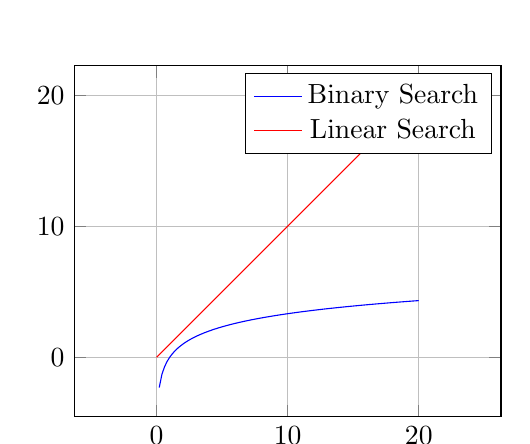
\begin{tikzpicture}

\begin{axis}[domain=0:20,
  samples=100,
  enlarge x limits=false,
  grid=both,
  no markers,
  axis equal]
  \legend{Binary Search, Linear Search}
\addplot {log2(\x)};
\addplot{\x};
\end{axis}
\end{tikzpicture}
\textbf{Figure 3}
\end{center}




It is clear that binary search is a more efficient algorithm than linear search. The key reason being that linear search is a brute force algorithm with complexity of $O(n)$, while binary search is a more complicated yet more efficient algorithm with complexity of $O(log_2(n))$. Linear search simply is checking every single item until it finds a match. The time it takes to find that item is somewhat random. For this reason, with a set size of 666 items, we can expect that on average it will take 333 tries  to get the right item, which is incredibly close to the actual result.

Binary search, however, is very stable. The reason being that, the only processing being done, is splitting the set into smaller and smaller pieces until it is small enough to know exactly where the item is. This splitting process is what gives Binary Search it's $O(log_2(n))$ complexity (see figure 3). 

\section{Hashing and Hash Tables}
\begin{center}
\textbf{ A Brief Explanation}
\end{center}

There are many complex ways to implement hashing using things such as one way hashes, nonces, public and private keys, and other things. Although, hashing can also be implemented quite simply. Hashing is the process of taking data, processing it in a certain way that returns a value that is not the same as the original data, and placing the data in a table in accordance to where it the value belongs. This certain way of processing is called a hash function.

As long as this hash function is known, and constant, the data can be retrieved from the table fairly quickly. Say for example the algorithm is simply the length of the string multiplied by six, we can just apply the same algorithm to the data we want to find and we will know where to look. Because of the likely chance that multiple data points will return the same hash value, we link together all of the like data points in lists called chains. Then, all the function would have to do is iterate over that list until it finds the correct data point.

\subsection{Overview of Functionality}

Being that a hash table is a conceptual thing, as opposed to the search functions which are static members of a class, it is useful to review the header file for the \texttt{HashTable} class.



\begin{addmargin}[-5em]{1em}
\begin{small}
\begin{minted}[linenos=true]{cpp}
#pragma once
#include "Node.h"
#include "Queue.h"
class HashTable {
public:
	static const int HASH_TABLE_SIZE = 250;
	Queue table[HASH_TABLE_SIZE];
	static int getHash(std::string item);
	void placeHashed(std::string item);
	void visualize();
	int getHashed(std::string items[], int chosenLen);
};
\end{minted}
\end{small}
\end{addmargin}
\begin{enumerate}
    \item \texttt{HASH\_TABLE\_SIZE} stores the defined length for the hash table.
    \item  The line \texttt{Queue table[HASH\_TABLE\_SIZE];} shows that the table itself is made up of \texttt{queue}s, a concept previously explored in a prior set of documentation.
    \item the \texttt{getHash()} function was made static so that a developer could use the hashing function without needing to create a hash table.
    \item \texttt{placeHashed()} simply takes in an item and places it in an array. This function does not take an array, as other than in the case of this demonstration, I did not believe that the table would be loaded all at once.
    \item \texttt{visualize()} simply allows the developer to see the data in the hash table in a simplified histogram view.
    \item \texttt{getHashed()} is used to retrieve items from the hash table.
\end{enumerate}
\subsection{Hash Table Functions}
\subsubsection{\texttt{getHash()}: Getting the Hash Value}

As explained above, this function is used to apply the hashing algorithm to a piece of data, in this case a string, and return a hash value to be used as the index in the hash table.
\begin{center}
    \textbf{Code Analysis}
\end{center}
\begin{addmargin}[-5em]{1em}
\begin{small}
\begin{minted}[linenos=true]{cpp}
int HashTable::getHash(std::string item)
{
	std::transform(item.begin(), item.end(), item.begin(), ::toupper);
	int sLen = item.length();
	int letterTotal = 0;
	for (int i = 0; i < sLen; i++)
	{
		char thisLetter = item[i];
		int thisValue = (int)thisLetter;
		letterTotal += thisValue;
	}
	int hashCode = (letterTotal * 1) % HASH_TABLE_SIZE;

	return hashCode;
}
\end{minted}
\end{small}
\end{addmargin}

\begin{enumerate}
    \item Normalize the string by setting the whole string to upper case.(line 3)
    \item For each character in the string, (line 6) take the integer value of that character (line 9) and add it to the \texttt{letterTotal} variable created previously(line 10).
    \item Take the modulus of the \texttt{letterTotal} mod \texttt{HASH\_TABLE\_SIZE}, the size of the table. Return this value. (lines 12,14)
\end{enumerate}




\subsubsection{\texttt{placeHashed()}: Putting in the Data}

Since the process of finding the hash value of an item is already defined, the \texttt{placeHashed()} function simply calls that function, and places it in the correct chain, or queue accordingly.
\begin{center}
    \textbf{Code Analysis}
\end{center}
\begin{addmargin}[-5em]{1em}
\begin{small}
\begin{minted}[linenos=true]{cpp}
void HashTable::placeHashed(std::string item)
{
	int hash = getHash(item);
	table[hash].enQueue(item);
}
\end{minted}
\end{small}
\end{addmargin}

\begin{enumerate}
    \item Get the hash value of the item by calling \texttt{getHash()} on the item.(line 3)
    \item Place the item in the \texttt{queue} defined by its hash value.(line 4)
\end{enumerate}

\subsubsection{\texttt{getHashed()}: Retrieving the data}

In order to retrieve the data, as covered previously, there is a very simple process. All the algorithm must do is apply the same hashing algorithm to the data that is desired to be retrieved, and search for it at the queue at the index defined by that hash value. 

\begin{addmargin}[-5em]{1em}
\begin{small}
\begin{minted}[linenos=true]{cpp}
int HashTable::getHashed(std::string items[], int chosenLen)
{
	std::cout << "--Retrieving hashed Data--" << std::endl;
	int tCount = 0;

	for (int i = 0; i < chosenLen; i++)
	{
		int count = 0;

		int hashLoc = getHash(items[i]);

		Queue chain = table[hashLoc];

		Node *n = chain.head;
	
		if (n->data == "")
		{
			std::cout << "If you're seeing this, the list is empty." << std::endl;
		}
		else
		{
			while (n->data != items[i])
			{
				count++;
				n = n->next;
			}

			std::cout << "Found it at place " << ++count << " in the chain." << std::endl;
			tCount += count; //take off the pre increment if uncommenting above line
		}
	}
	int avg = tCount / chosenLen;
	return avg;
}

\end{minted}
\end{small}
\end{addmargin}

\begin{center}
    \textbf{Code Analysis}
\end{center}
\begin{enumerate}
    \item For each item in the chosen items list (line 6) start by initializing the temporary \texttt{count} variable, and getting the hash value of the current items being looked for.
    \item Ensure that the queue is not empty before proceeding. (line 18)
    \item Iterate over the queue until the desired item is found, adding one to the \texttt{count} variable each time. (lines 22-26)
    \item Announce the place in the chain, and add on the temporary \texttt{count} to the \texttt{tCount}, which holds the total count.
    \item Compute and return the average number of comparisons to get to the desired elements, including the correct one, by dividing the \texttt{tCount} by the amount of items searched for.(line 32)
\end{enumerate}



\subsubsection{\texttt{visualize()}: Seeing What Is In The Table }

This function iterates through each \texttt{queue} in the table, adding an asterisk for every element it sees. With the careful placement of some 
\texttt{std::cout << std::endl}s, it creates a histogram of the data.

\begin{center}
    \textbf{Code Analysis}
\end{center}
\begin{addmargin}[-5em]{1em}
\begin{small}
\begin{minted}[linenos=true]{cpp}
void HashTable::visualize()
{
	std::cout << "---visualizing your data---" << std::endl;

	for (int i = 0; i < HASH_TABLE_SIZE; i++)
	{ //getting the data

		if (table[i].head == nullptr)
		{
			std::cout << i << "|" << std::endl;

	
		}
		else
		{
			std::cout << i << "|";
			Node *start = table[i].head;
			while (start != nullptr)
			{
				std::cout << "*";
				start = start->next;
			}
			std::cout << std::endl;
		}
	}
}
\end{minted}
\end{small}
\end{addmargin}

\begin{enumerate}
    \item For each \texttt{queue} in the table (line 5), iterate over the \texttt{queue}, or chain.
    \item Check that the chain is populated, and if it is not, print a blank "bar".(lines 8-13)
    \item If the chain is not empty, begin by placing the "x axis" line. Then, grab the head pointer of the chain (lines 16,17)
    \item Iterate over the chain, adding an asterisk for every \texttt{node} passed, and continuing until the last element is found (lines 18-22)
    \item End the current "bar" and continue to the next chain.
\end{enumerate}
\subsection{Asymptotic Running Time Analysis Of Hash Table Functions}

Generally speaking, searching in a hash table has complexity of $O(1)$. The reason being that it is very unlikely that two items will have the same hash value. Also, there is the simple fact that by knowing the hash value, you have a very good idea of where the item is, it's just a matter of getting to your element in the array. Here, the running time turns into a linear search, which is $O(n)$. To find the complexity we start by computing our load factor, and adding in the 1 for the constant time to hash and move to the right  place. With this, we see that our complexity is $O(1+1.67)$, or $O(2.67)$.

As a side note, getting the hash value and placing the hash value are also constant time operations. Getting the hash value will always take the same amount of time, and all \texttt{placeHashed()} is doing is \texttt{enQueue()}ing that element, which is also constant time.

\section{ \texttt{Main.cpp}: Putting it All Together}

Lastly, There is the implementation of all of these algorithms. Due to the fact that it has been covered multiple times in previous documents, the process of setting up the array from the text file will not be covered here. The only modification is that once the array is loaded, \texttt{mergeSort()} is called on the array in order to sort it.

\subsection{\texttt{hashTheTable()}: Loading The Table In One Batch}

This function simply iterates over the main array of elements, applys the hashing algorithm, and places it accordingly using the \texttt{placeHashed()} function all in one step. Then once all is completed, \texttt{visualize()} the data.

\begin{addmargin}[-5em]{1em}
\begin{small}
\begin{minted}[linenos=true]{cpp}
 void hashTheTable(std::string arr[], int len, HashTable * tab) { 
 	//HashTable* tab = new HashTable();
 	for (int i = 0; i < len; i++) {
 		tab->placeHashed(arr[i]);
 	}
 	tab->visualize();
	
 }
\end{minted}
\end{small}
\end{addmargin}

\subsection{\texttt{main()}: Running the Code}

Here is where all of the pieces come together and are ran by the program.
\begin{center}
    \textbf{Code Analysis}
\end{center}
\begin{addmargin}[-5em]{1em}
\begin{small}
\begin{minted}[linenos=true]{cpp}
int main()
{
	setup();


	std::string items[CHOSEN_LEN];
	Search::randPick(arr, items,LEN,  42);
	int linAvg = Search::linSearch(arr, LEN, items, CHOSEN_LEN);
	int binAvg = Search::binSearch(arr, LEN, items, 42);
	std::cout << "Linear Search:||: Average comparisons to get a hit: " << linAvg << std::endl;
	std::cout << "Binary Search:||: Average comparisons to get a hit: " << binAvg  << std::endl;
	HashTable * hTable = new HashTable();
	hashTheTable(arr, LEN, hTable);
	int tCount = hTable->getHashed(items, CHOSEN_LEN);
	std::cout << "Average " << tCount << " comparisons to retrieve each item." << std::endl; 
}

\end{minted}
\end{small}
\end{addmargin} 

\begin{enumerate}
    \item set up the table.( line 3)
    \item Initiate the items array, and populate it with random items using the \texttt{randPick} function.(lines 9, 10)
    \item Run linear and binary search, and print out the average comparisons for each. (lines 11-14)
    \item Create the hash table. (line 15)
    \item run the \texttt{hashTheTable()} function on the hash table to load it with data. (line 16)
    \item Retrieve the list of random items from the main list, and print the average comparisons to find each one (lines 17-18)
\end{enumerate}


\section{Results and Conclusion}

The results of these functions have been listed throughout this document, although here is a consise summation of the data collected along with a graph of all of the complexities.

\begin{center}
{\rowcolors{2}{gray!50}{white!100}
 \begin{tabular}{||c c c c||} 
 \hline
 Search Algorithm & Aveargage Comparisons  & Complexity/ $O()$\\ [0.5ex] 
 \hline\hline
 Linear Search& 332 &  $O(n)$\\ 
 \hline
 Binary Search& 8 & $O(log_2(n))$\\
 \hline
 getHashed() & 2 & $O(2.67)$\\
 \hline
 placeHashed() \& getHash() & - & $O(1)$ \\
 \hline
\end{tabular}
}
\textbf{Figure 4}
\end{center}
\begin{center}
    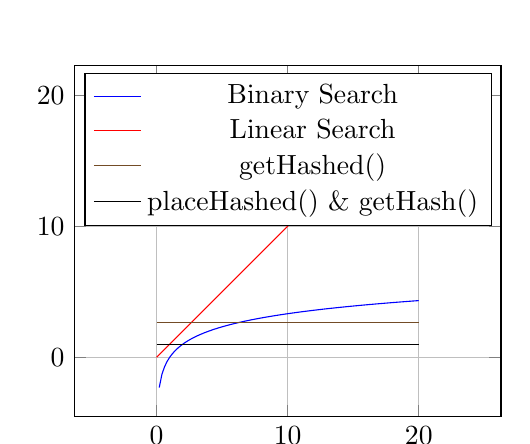
\begin{tikzpicture}

\begin{axis}[domain=0:20,
  samples=100,
  enlarge x limits=false,
  grid=both,
  no markers,
  axis equal]
  \legend{Binary Search, Linear Search, getHashed(), placeHashed() \& getHash()}
\addplot {log2(\x)};
\addplot{\x};
\addplot{2.67};
\addplot{1};
\end{axis}
\end{tikzpicture}
\textbf{Figure 5}
\end{center}

\textbf{Closing Thoughts}

At the start, I was sure that this assignment would be no trouble at all. Simple arrays, simple enough functions, what could go wrong? But yet again, the concept of pointers and references, and view access rights caused me to completely give up on my efforts. Thankfully, I remembered that at the point of my previous commit, I was not having this error, so I hedged my bets, downloaded the previous commits version of the repository, and started over. With this, along with using g++ to debug, the problem was solved in no time.
\newline

as a wise person once said, "
give a person a program and they'll be
frustrated for a day, teach a person to
program and they'll be frustrated for the
rest of their life.".
 \vspace{.5em}
{\textit{\color{red}\huge{\{S.A.\}}}}
\vspace{1em}

\newpage
\begin{center}
    \textbf{References}
\end{center}



Williams Jr., L. F. (2020, October 20). Binary search algorithm. 
Retrieved October 29, 2020, from https://en.wikipedia.org/wiki/Binary\_search\_algorithm

\end{document}
